\documentclass[11pt]{article}
\usepackage[utf8]{inputenc}\usepackage[T1]{fontenc}
\usepackage{amsmath,amssymb,amsthm}\usepackage[margin=1in]{geometry}
\usepackage{graphicx}\usepackage{booktabs}\usepackage{multirow}\usepackage{enumitem}
\usepackage[hidelinks]{hyperref}
\newtheorem{proposition}{Proposition}

\title{A Second-Order Conditional Singular Series for Twin-Prime Gaps\\
on the $6N$ Skeleton: the Spatial-Compression Penalty\\
and a Residual Shield-Gain Term}
\author{Ruqing Chen\\
\small GUT Geoservice Inc., Montreal, Quebec, Canada\\
\small \texttt{ruqing@hotmail.com}}
\date{\today}

\begin{document}
\maketitle

\begin{abstract}
Part~III gave a first-order conditional singular series
$\mathfrak{S}_{2,\omega}(d)\approx C_2(d)L_\omega(d)$ for the twin-prime gap
distribution on the $6N\pm1$ skeleton, reproducing the $\omega$-trends of the
gaps $30,42,60$ and the direction of the collapse of $210$, but leaving a stable
high-$\omega$ residual on $210$ (observed $0.41$ where the first-order series
predicts $0.62$ at $\omega=6$). Here we identify the second-order term
responsible. The first-order series treats the primes $q\nmid N$ by their
unconditional Hardy--Littlewood factor; but conditioning on $q\nmid N$ is itself
a constraint---it removes the residue $N\equiv0$ and crowds $N$ into the
remaining $q-1$ classes, where the same fatal residues now occupy a larger
fraction. This \emph{spatial-compression penalty}
$\mathrm{pen}_q(d)=\frac{(q-1-k_q)/(q-1)}{(q-k_q)/q}<1$ lowers the survival of
factor-rich centres on gaps locked by small primes. Evaluated on the
$23{,}988{,}173$ twin centres of $S_{10}$ with each centre's real factor set,
the second-order series closes the $210$ residual essentially completely (at
$\omega=6$, observed $0.413$, second order $0.426$, against first order $0.357$),
across all strata. It also corrects the direction on $42$ but only partially:
about half of the high-$\omega$ rise of $42$ remains unexplained, an effect we
attribute to a complementary \emph{factor-coincidence shield gain} on the
$q\mid N$ side (the gap $42$ contains the factor $7$) that the compression
penalty does not capture. The long-gap residual of Part~III is thus resolved;
the short-gap residual is sharpened into a named two-centre open problem. No
claim is made about the infinitude of twin primes or any $k$-tuple conjecture.
\end{abstract}

\section{The first-order blind spot}

Part~III~\cite{ChenIII} wrote the first-order conditional singular series as
$\mathfrak{S}_{2,\omega}(d)\approx C_2(d)\,L_\omega(d)$, where for each prime
$q\mid N$ the congruence-lockdown rule forbids the gap residues
$d\equiv\pm6^{-1}\pmod q$, and each prime $q\nmid N$ contributes its
\emph{unconditional} Hardy--Littlewood factor. The residual on $210$ showed this
last step to be incomplete: at high $\omega$ the observed preference fell well
below the first-order prediction.

The blind spot is the treatment of $q\nmid N$. In a stratum of factor-rich
centres, ``$q\nmid N$'' is not a neutral background event but a constraint. Fix
a prime $q$ that does not lock the gap $d$ (so $q\nmid 6d\pm1$, and the fatal
residue set of $d$ modulo $q$ does not contain $0$). Unconditionally, $N$ ranges
over all $q$ classes and the joint twin survival omits the $k_q$ fatal residues,
giving a factor $\propto (q-k_q)/q$. But conditioning on $q\nmid N$ deletes the
class $N\equiv0$: $N$ now ranges over only $q-1$ classes, while the same $k_q$
fatal residues persist (none of them is $0$). The conditional survival is
therefore $\propto (q-1-k_q)/(q-1)$.

\begin{proposition}[spatial-compression penalty]\label{prop:pen}
For a prime $q$ that does not lock the gap $d$, conditioning on $q\nmid N$
multiplies the per-$q$ twin-survival factor by
\[
  \mathrm{pen}_q(d)\;=\;\frac{(q-1-k_q)/(q-1)}{(q-k_q)/q}
  \;=\;\frac{q\,(q-1-k_q)}{(q-1)(q-k_q)}\;<\;1,
\]
where $k_q$ is the number of fatal residues of $d$ modulo $q$ (the classes
$N\equiv\pm6^{-1},\,-d\pm6^{-1}$, none equal to $0$ since $q$ does not lock $d$).
\end{proposition}

The penalty is strictly below $1$: forced off the class $N\equiv0$, the centre
is crowded into a smaller space where the fatal residues are proportionally
denser, so its twin survival drops. This is the second-order effect omitted at
first order.

\section{Second-order series and confrontation with $S_{10}$}

Including the penalty, the second-order conditional weight of a gap $d$ at a
real centre $N$ with small-prime factor set $Q$ is
\[
  w^{(2)}(d,N)=C_2(d)\cdot \mathbf{1}\{\text{no }q\in Q\text{ locks }d\}\cdot
  \prod_{\substack{q\notin Q,\ q\,\nmid\,(6d\pm1)}}\mathrm{pen}_q(d).
\]
We evaluate this over the $23{,}988{,}173$ twin centres of $S_{10}$ using each
centre's true factor set (no independence or uniform-combination assumption),
aggregate by $\omega_{>3}(N)$, and compare to the observed preference and to the
first-order series (Fig.~\ref{fig:so}, Table~\ref{tab:so}).

\begin{figure}[h]\centering
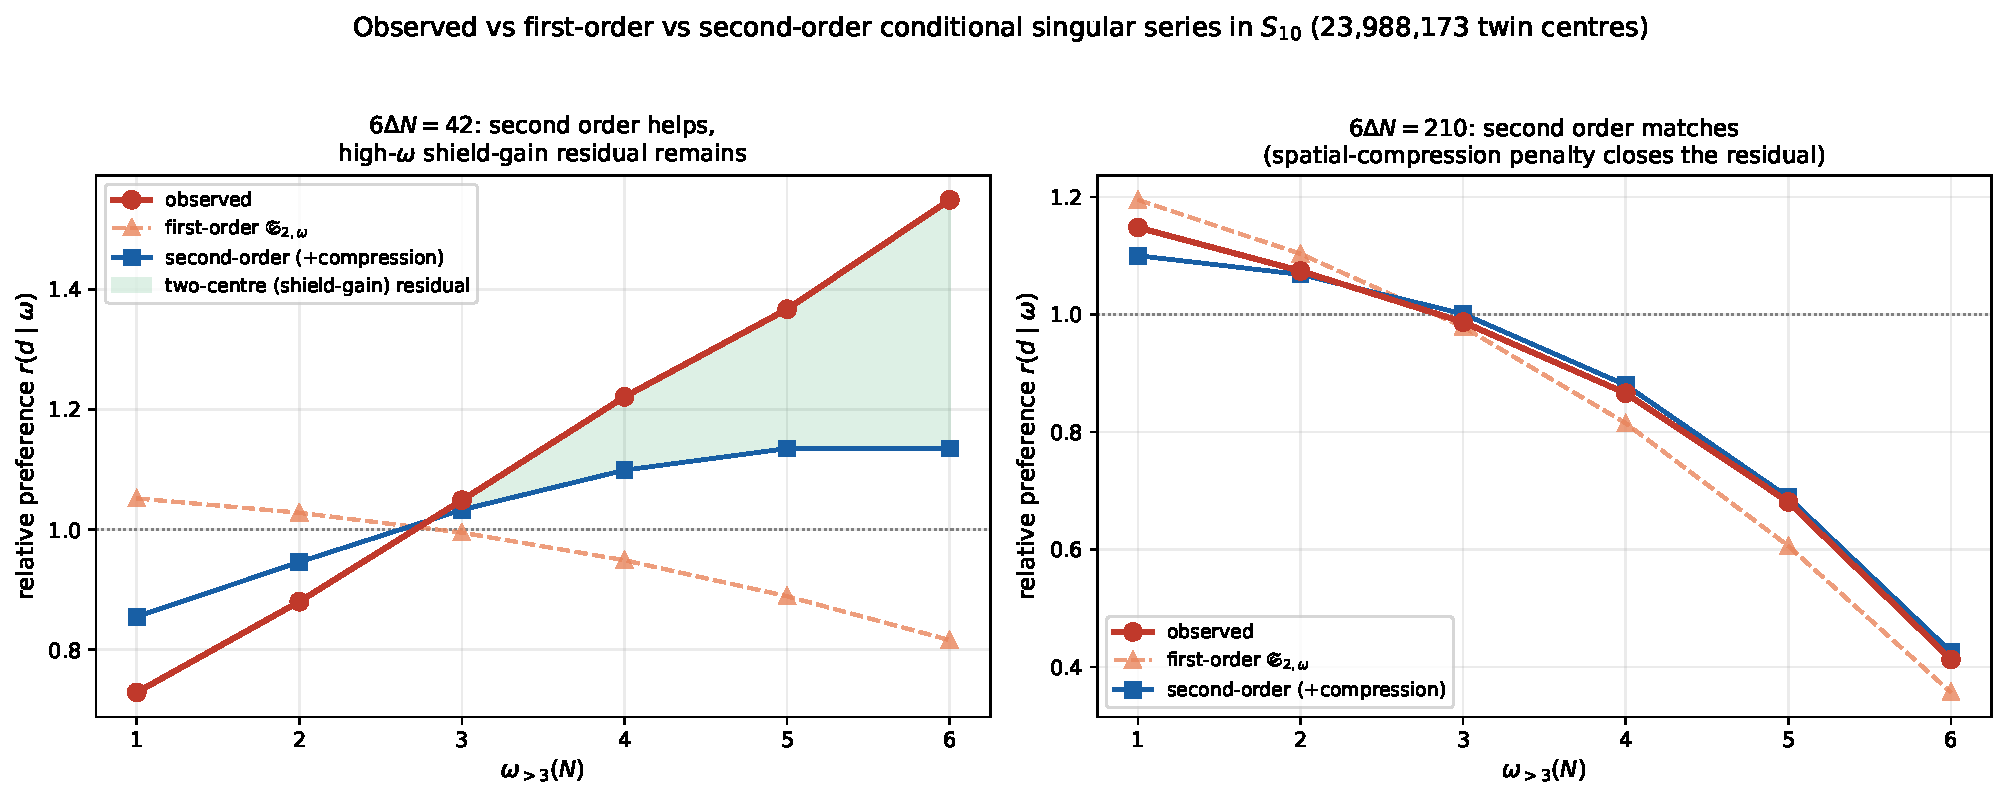
\includegraphics[width=\textwidth]{fig_paper4_second_order.pdf}
\caption{Observed (red), first-order (orange dashed), and second-order (blue)
conditional singular series in $S_{10}$. \textbf{Right ($6\Delta N=210$):} the
spatial-compression penalty closes the first-order residual at every stratum.
\textbf{Left ($6\Delta N=42$):} the penalty corrects the direction and recovers
about half of the high-$\omega$ rise, but a residual (shaded) remains, attributed
to a complementary shield-gain term.}
\label{fig:so}
\end{figure}

\begin{table}[h]\centering
\begin{tabular}{llcccccc}
\toprule
$6\Delta N$ & model & $\omega{=}1$ & 2 & 3 & 4 & 5 & 6\\
\midrule
\multirow{3}{*}{$210$}
 & observed     & 1.15 & 1.07 & 0.99 & 0.87 & 0.68 & 0.41\\
 & first-order  & 1.20 & 1.10 & 0.98 & 0.82 & 0.61 & 0.36\\
 & second-order & 1.10 & 1.07 & 1.00 & 0.88 & 0.69 & 0.43\\
\midrule
\multirow{3}{*}{$42$}
 & observed     & 0.73 & 0.88 & 1.05 & 1.22 & 1.37 & 1.55\\
 & first-order  & 1.05 & 1.03 & 1.00 & 0.95 & 0.89 & 0.82\\
 & second-order & 0.86 & 0.95 & 1.03 & 1.10 & 1.14 & 1.14\\
\bottomrule
\end{tabular}
\caption{Observed, first-order, and second-order $r(d\mid\omega)$ in $S_{10}$.
For $210$ the second order tracks the observation at every stratum; for $42$ it
corrects the direction but stalls near $1.14$ while the observation continues to
$1.55$.}
\label{tab:so}
\end{table}

\paragraph{Long gap $210$: resolved.}
The lock primes of $210$ are $11,19$ (since $6\cdot35-1=209=11\times19$). At high
$\omega$, surviving centres are precisely those forced to avoid $11$ and $19$, so
the compression penalty acts on exactly these primes
($\mathrm{pen}_{11}\approx0.94$). The second-order series reproduces the observed
collapse at every stratum (Table~\ref{tab:so}, top), closing the Part~III
residual.

\paragraph{Short gap $42$: corrected in direction, residual remains.}
The lock primes of $42$ are $41,43$ (both prime, since $6\cdot7\mp1=41,43$),
which are rarely divisors of a centre, so $42$ suffers little lockdown and little
compression---correctly, the second-order series turns the (wrongly decreasing)
first-order curve upward. But it stalls near $1.14$ while the observation reaches
$1.55$ (Table~\ref{tab:so}, bottom). About half of the high-$\omega$ rise is
still unexplained.

\paragraph{Normalisation note.}
The relative preferences $r(d\mid\omega)$ here are normalised \emph{model-internally}:
each of the three curves (observed, first-order, second-order) is divided by its
own $\omega$-merged mean, so that the average over strata is unity. This differs
from the global $C_2\times$envelope baseline used in Part~III; the two
conventions differ by a constant scaling per gap and per model, which shifts the
absolute level but not the gradient in $\omega$ or the relative size of the
residuals. We use the model-internal convention because the object of interest
here is precisely the per-stratum departure of each model from the observation,
which it isolates cleanly; readers comparing absolute $\omega=1$ levels across
Parts~III and~IV should account for this constant offset.

\section{The residual: the single-centre limitation}

It is important to be exact about what the second-order series is and is not.
Proposition~\ref{prop:pen} is a \emph{single-centre} condition: it conditions on
the factorisation of the left centre $N$, and treats the right centre $N+d$ as
independent of $N$ given that conditioning. This is an idealisation. The two
centres differ by a fixed $d$, so modulo any prime $q$ their residues are
\emph{strongly correlated} ($N+d\equiv N+d$, deterministically), not
independent. The genuinely missing piece is therefore not ``a further order'' on
top of an exact formula, but the \emph{two-centre correlation} that the
single-centre second-order series omits by construction.

This omission is mild for $210$ and severe for $42$, which is exactly the pattern
observed. For $210$, the lock primes $11,19$ rarely divide both $N$ and $N+210$,
so the single-centre treatment is close to correct and the residual is closed
(Table~\ref{tab:so}). For $42$ the correlation is strong and favourable: $42=6
\cdot7$, and $7$ is one of the small primes a factor-rich centre typically
carries. When $7\mid N$, both centres are shielded against $7$ simultaneously,
since $6N\pm1\equiv\pm1$ and $6(N+42)\pm1\equiv\pm1\pmod 7$ alike---a
\emph{factor-coincidence shield gain} in which the gap's own factor $7$ aligns
with the centre's. The single-centre series, conditioning only on $N$, does not
carry this joint two-centre shielding, and so under-predicts the rise of $42$.

\begin{quote}
\textbf{Open problem (two-centre correlation).} The present second-order series
is limited to a single-centre condition. Derive the two-centre conditional
singular series that retains the correlation between the factorisations of $N$
and $N+d$ modulo each $q$ --- in particular the factor-coincidence shield gain
when a prime dividing the centre also divides the gap (e.g.\ $7\mid N$ for
$d=7$) --- and test whether it accounts for the residual rise of $42$ (observed
$1.55$ versus single-centre second-order $1.14$ at $\omega=6$ in $S_{10}$). The
shield-gain mechanism above is at present only a \emph{qualitative} hypothesis;
unlike the compression penalty it has not been reduced to a verified closed-form
factor. Establishing it quantitatively would complete the conditional singular
series beyond the single-centre approximation.
\end{quote}

\section{Conclusion}

We identified the second-order term of the conditional twin-gap singular series:
a spatial-compression penalty arising because conditioning on $q\nmid N$ crowds
the centre into $q-1$ classes. Evaluated on $2.4\times10^{7}$ twin centres, it
closes the long-gap ($210$) residual that Part~III left open, at every stratum.
It corrects the direction of the short-gap ($42$) trend but recovers only about
half of its high-$\omega$ rise. The remainder is not a missing ``further order''
on top of an exact formula: the second-order series is by construction a
\emph{single-centre} condition, conditioning on the factorisation of $N$ while
treating $N+d$ as independent. The two centres are in fact correlated modulo each
prime, and the unexplained rise of $42$ reflects a favourable two-centre
coincidence (the gap's factor $7$ shielding both centres when $7\mid N$), which
the single-centre series omits. We pose this two-centre conditional singular
series, and the quantitative form of the shield gain, as the open problem. The
picture is layered and explicit: first-order lockdown (absolute exclusion when
$q\mid N$ locks the gap), second-order single-centre compression (survival drop
when $q\nmid N$), and a remaining two-centre correlation (the shield gain, still
only a qualitative hypothesis). As throughout this series, we make no claim about
the infinitude of twin primes or any $k$-tuple conjecture; this is a conditional,
factor-resolved refinement of the Hardy--Littlewood gap heuristic, demonstrated
empirically and offered with its open remainder.

\paragraph{Data and code availability.}
The scan, the first- and second-order series evaluation, and the figure code are
openly available~\cite{repo}; the $S_{10}$ twin count $23{,}988{,}173$ matches
Part~I.

\begin{thebibliography}{9}
\bibitem{ChenI} R.~Chen, \emph{Prime distribution on the $6N$ skeleton} (Part~I),
Zenodo, doi:10.5281/zenodo.20470367 (2026).
\bibitem{ChenII} R.~Chen, \emph{Prime gaps on the $6N$ skeleton: an
$\omega$-dependent shift and a congruence-lockdown mechanism} (Part~II), Zenodo,
doi:10.5281/zenodo.20477664 (2026).
\bibitem{ChenIII} R.~Chen, \emph{A first-order conditional singular series for
twin-prime gaps on the $6N$ skeleton, and its second-order residual} (Part~III),
Zenodo, doi:10.5281/zenodo.20498668 (2026).
\bibitem{HL} G.~H.~Hardy, J.~E.~Littlewood, \emph{Partitio Numerorum III}, Acta
Math.\ \textbf{44} (1923), 1--70.
\bibitem{repo} R.~Chen, \emph{$6N$ twin-prime conditional singular series: data
and code}, \url{https://github.com/Ruqing1963/6N-twin-prime-second-order-residual} (2026).
\end{thebibliography}

\end{document}
